\label{sumgen}
\subsection{Ranking \& Selection}
\label{ranking}
As in \cite{DBLP:conf/cikm/MaSYC12} and \cite{DBLP:conf/ecir/AkerKBPBHG16}, clusters are selected by the number of comments they contain. Thus, the scoring function is defined as $f(C^{t_i}) = |C^{t_i}|$, i.e. assigns each cluster the number of its comments. The ten largest clusters are selected for summary.\par
Comments are selected as a summary of each selected cluster.
The objective of ranking comments is to find the comments which represent the topic of the cluster concisely. Thus, a ranking mechanism should rank comments highest which are closest to the topic of the cluster without being redundant. As Maximal Marginal Relevance (MMR) \cite{Carbonell:1998:UMD:290941.291025} aims for both, it is selected for this thesis.
MMR in the context of the presented thesis is defined according to \cite{Carbonell:1998:UMD:290941.291025}.
\begin{definition}{Maximal Marginal Relevance}
Let $C^{t_i} = \{c \in C|t_i = \argmax_{t \in T} P(t|c)\}$ be a set of comments sharing a topic $t_i \in T$, where $T$ denotes the set of all topics. Let $S$ be a set of already selected comments, $q$ denote a set of words representing $t_i$ and $s_1$ and $s_2$ be two similarity measures. Then MMR is defined as:
\begin{equation}
\text{MMR} = \argmax_{c_i \in C^{t_i} \setminus S} \left[\lambda\left(s_1(c_i,q)-(1-\lambda)\max_{c_j \in S} s_2(c_i,c_j)\right)\right]
\end{equation}
Here, $\lambda$ decides about the diversity of the ranking effort \cite{Carbonell:1998:UMD:290941.291025}.
It is easy to see that for $\lambda = 1$, the ranking is entirely based on similarity to the query. A larger $\lambda$ possibly returns more redundant information close to the query, while a smaller $\lambda$ returns a sample of information around the query \cite{Carbonell:1998:UMD:290941.291025}. That is, a smaller $\lambda$ returns a more diverse set of comments while a larger $\lambda$ returns comments very close to the topic representation $q$.
\end{definition}
In this thesis, we choose $\lambda = 0.8$ as reported suitable for comments in \cite{DBLP:conf/cikm/MaSYC12}.
Furthermore, we choose cosine similarity of TF-IDF vector representations for both similarity measures.
For topic representation, the most likely words by topic-word distribution of a topic model are used, because it assigns high probabilities to words likely to be present in a document when it is known to talk about the topic. Thus, such words are descriptive of the topic. Again, for the MCL such a distribution does not exist but a topic model can be trained on the comments (and articles) of each topic cluster found by MCL with a topic number of 1 to obtain a topic-word distribution. In the end, highest scored comments of positive and of negative sentiment are chosen as a summary of each selected topic cluster.

\subsection{Sentiment analysis}
Selection requires the sentiment of each considered comment to be known. Therefore, polarity of comments is calculated using the pretrained VADER \cite{DBLP:conf/icwsm/HuttoG14} sentiment analysis model of NLTK. Each comment is assigned a valence score indicating positive, neutral or negative sentiment. For more details on sentiment analysis and the VADER model, the reader is kindly referred to \cite{DBLP:conf/icwsm/HuttoG14}. 

\subsection{Visualization}
\label{sample}
\begin{figure}[H]%
\label{sumfig}
\centering
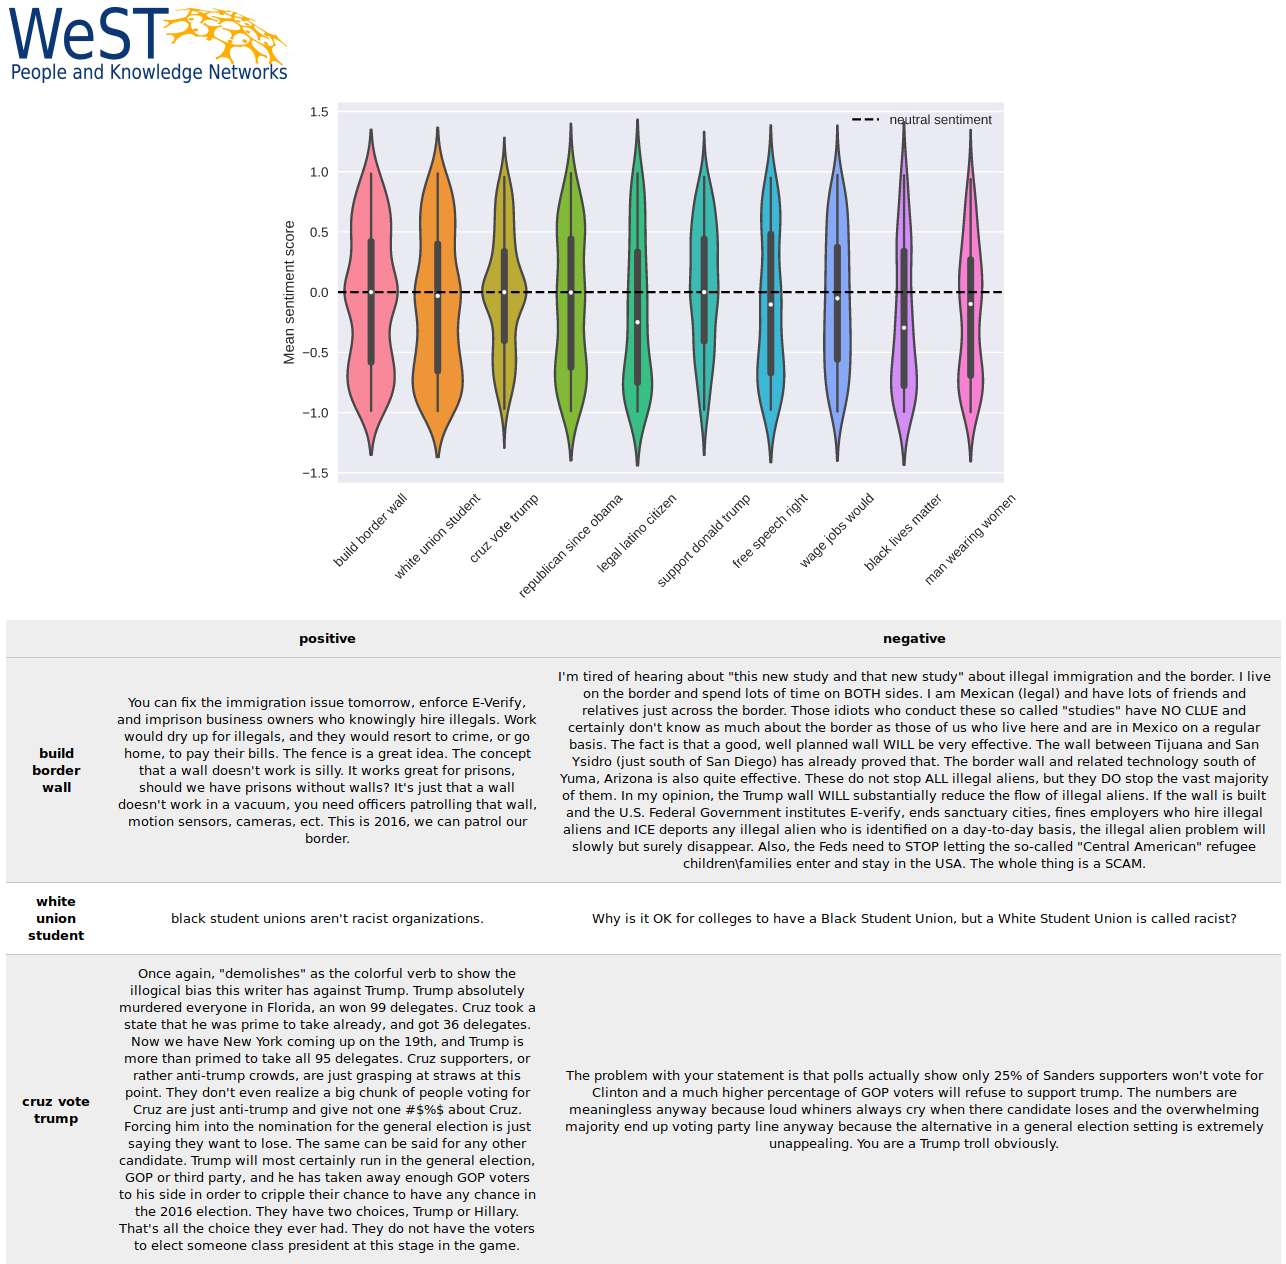
\includegraphics[width=\textwidth]{img/sample_summary.png}%
\caption{A sample summary of dataset \#3 created using HMDP, the oulined labeling and MMR with $\lambda = 0.8$. The table is cut off for brevity; the entire page shows all 10 selected topics.}
\end{figure}
In accordance with the results of a study of summary design for online debates carried out by Sanchan et al. \cite{DBLP:journals/polibits/SanchanBA16}, a combination of chart and side-by-side summary in the form of a table is chosen.
We choose the violin plot as chart, since it combines the information of a boxplot with a probability density estimate.The distribution of sentiment across comments is plotted with the chart indicating how many comments were assigned the topic in general and by polarity. Since all selected topics are plotted against each other and the violin areas are scaled by the number of contained comments, this enables a quick comparison between the significance of topics. Furthermore, one can get a brief overview over the overall reception of it.
For each topic, the comments selected as outlined in the previous subsection are shown in a table. This allows for a quick overview of positive and negative aspects.
\clearpage